\documentclass{article}
\usepackage[utf8]{inputenc}

\usepackage{amsmath,amsbsy,amssymb,amsthm}
\usepackage{multirow,multicol,tabularx,booktabs}
\usepackage{graphicx,placeins,color,url}
\usepackage{bbm,bm}
\usepackage[ruled]{algorithm2e}
\usepackage[shortlabels]{enumitem}
\usepackage{mathrsfs}
\usepackage{textcase}

\usepackage[top=2.5cm,bottom=2.5cm, right=2.5cm,left=2.5cm]{geometry}
\usepackage[hidelinks]{hyperref}
\renewcommand{\baselinestretch}{1.5}

% For the graphs
\usepackage{tikz}
\usetikzlibrary{arrows,arrows.meta,shapes.arrows,positioning,calc}

\newtheorem{conj}{Conjecture}[section]
\newtheorem{thm}[conj]{\bf Theorem}
\newtheorem{defi}[conj]{\bf Definition}
\newtheorem{cor}[conj]{\bf Corollary}
\newtheorem{prop}[conj]{\bf Proposition}
\newtheorem{lemma}[conj]{\bf Lemma}
\newtheorem{rem}[conj]{\bf Remark}
\newtheorem{cond}[conj]{\sc Condition}
\newtheorem{example}[conj]{\bf Example}
\newtheorem{assumpt}{\bf Assumption}



%\newcommand{\JSH}{\color{blue}}
\newcommand{\Alexis}{\color{red}}

\def\eps{\varepsilon}


\def\bar{\overline}
\def\SN{{\N}(0,1)}
\def\sign{{\; \text{sign}}}

\def\implies{\Longrightarrow}

\def\to{\rightarrow}
\def\To{\longrightarrow}
\def\weakly{\buildrel {W} \over \longrightarrow}
\def\inprobto{{\buildrel \mathbb P \over \longrightarrow \,}}
\def\equalindistr{\buildrel {d} \over =}
\def\indistrto{\buildrel {D} \over \longrightarrow}
\newcommand{\eqinfty}[1]{{\buildrel {#1 \to \infty} \under =}}
\def\simiid{\buildrel {\text{i.i.d.}} \over \sim}

\def\Bias{\operatorname{Bias}}
\def\IB{\operatorname{IBias}^2}
\def\Cov{\operatorname{Cov}}
\def\Var{\operatorname{Var}}
\def\IVar{\operatorname{IVar}}
\def\MSE{\operatorname{MSE}}
\def\MISE{\operatorname{MISE}}
\def\Med{\operatorname{Med}}
\def\supp{\operatorname{supp}}
\def\JS{\operatorname{JS}}
\def\Tr{\operatorname{Tr}}
\def\Card{\operatorname{Card}}

\def\TV{\operatorname{TV}}
\def\KL{\operatorname{KL}}
\def\Jac{\operatorname{Jac}}
\def\Det{\operatorname{Det}}
\def\Rank{\operatorname{Rank}}
\def\Diag{\operatorname{Diag}}
\def\Vect{\operatorname{Vect}}
\def\dim{\operatorname{dim}}
\def\mc{\operatorname{mc}}

\def\Lap{\operatorname{Lap}}
\def\Pois{\operatorname{Pois}}
\def\Exp{\operatorname{Exp}}
\def\Ber{\operatorname{Ber}}
\def\om{\omega}
\def\EssSup{\operatorname{ess \, sup}}

\def\Ac{\mbox{$\mathcal A$}}
\def\Bc{{\mathscr B}}
\def\Cc{{\mathscr C}}
\def\Dc{\mbox{$\mathcal D$}}
\def\Ec{{\mathscr E}}
\def\Fc{{\mathscr F}}
\def\Gc{{\mathscr G}}
\def\Hc{\mbox{$\mathcal H$}}
\def\Ic{\mbox{$\mathcal I$}}
\def\Jc{\mbox{$\mathcal J$}}
\def\Kc{\mbox{$\mathcal K$}}
\def\Lc{\mbox{$\mathcal L$}}
\def\Mc{{\mathcal M}}
\def\Nc{\mbox{$\mathcal N$}}
\def\Oc{\mbox{$\mathcal O$}}
\def\Pc{\mbox{$\mathcal P$}}
\def\Qc{\mbox{$\mathcal Q$}}
\def\Rc{\mbox{$\mathcal R$}}
\def\Sc{{\mathcal S}}
\def\Tc{{\mathcal T}}
\def\Uc{\mbox{$\mathcal U$}}
\def\Vc{\mbox{$\mathcal V$}}
\def\Wc{\mbox{$\mathcal W$}}
\def\Xc{{\mathcal X}}
\def\Yc{\mbox{$\mathcal Y$}}
\def\Zc{{\mathcal Z}}

\def\AA{{\mathbb A}}
\def\BB{{\mathbb B}}
\def\CC{{\mathbb C}}
\def\DD{{\mathbb D}}
\def\FF{{\mathbb F}}
\def\Gb{{\mathbb G}}
\def\HH{{\mathbb H}}
\def\II{{\mathbb I}}
\def\LL{{\mathbb L}}
\def\NN{{\mathbb N}}
\def\GG{{\mathbb G}}
\def\QQ{{\mathbb Q}}
\def\Rb{{\mathbb R}}
\def\Vb{{\mathbb V}}
\def\WW{{\mathbb W}}
\def\Zb{\mbox{$\mathbb Z$}}

%\def\Var{{\mathbb{V}\mathrm{ar}}}

\def\a{ {\bf a}}
\def\e{ {\bf e}}
\def\t{ {\bf t}}
\def\u{ {\bf u}}
\def\v{ {\bf v}}
\def\x{ {\bf x}}
\def\y{ {\bf y}}
\def\z{ {\bf z}}

\def\S{ {\bf S}}
\def\U{ {\bf U}}
\def\W{ {\bf W}}
\def\X{ {\bf X}}
\def\Y{ {\bf Y}}
\def\Z{ {\bf Z}}

\def\1{\mathbbm{1}}
\def\floorbeta{{\lfloor \beta \rfloor}}
\def\ceilbeta{{\lceil \beta \rceil}}

\def\Mk{{\mathfrak{M}}}
\def\Sigmam{\mathfrak{S}_m}
\def\Om{\mathcal{O}_m}
\def\proj{{\mathfrak{p}}}
\def\image{{\rm Im}}
\def\ballmA{{{\mathscr B}_m(A)}}
\def\support{{\rm Supp}}

\def\wh{\widehat}
\def\wt{\widetilde}
\def\ol{\overline}


\title{Codivergences and information matrices}
\author{Alexis Derumigny\footnote{Department of Applied Mathematics, Delft University of Technology, Mekelweg 4, 2628 CD Delft, The Netherlands. {\small {\em Email:} \texttt{A.F.F.Derumigny@tudelft.nl}}} \ and Johannes Schmidt-Hieber\footnote{University of Twente, Drienerlolaan 5, 7522 NB Enschede, The Netherlands. {\small {\em Email:} \texttt{a.j.schmidt-hieber@utwente.nl}} \newline The research has been supported by the NWO/STAR grant 613.009.034b and the NWO Vidi grant VI.Vidi.192.021.}}
\date{\today}


\begin{document}

\maketitle

\begin{abstract}
We propose a new concept of codivergence, which quantifies the similarity between two probability measures $P_1, P_2$ relative to a reference probability measure $P_0$. In the neighborhood of the reference measure $P_0$, a codivergence behaves like an inner product between the measures $P_1-P_0$ and $P_2-P_0$. Two specific codivergences, the $\chi^2$-codivergence and the Hellinger codivergence are introduced and studied. We derive explicit expressions for several common parametric families of probability distributions.
For a codivergence, we introduce moreover the divergence matrix as an analogue of the Gram matrix. It is shown that the $\chi^2$-divergence matrix satisfies a data-processing inequality.
\end{abstract}

{\bf Keywords:} Divergence, chi-square divergence, Hellinger affinity, Gram matrix.

{\bf MCS 2020:} 62B11, 46E27, 15A63.

\section{Introduction}

One of the objectives of information geometry is to measure distances or angles in statistical spaces, usually for parametric models.
This is often done by the use of a divergence, generating a Riemannian manifold structure on the considered space of distributions, see \cite{amari2016information,ay2017information,nielsen2020elementary}.
Divergences between probability measures quantify a certain notion of difference between them. Divergences are in general not symmetric, as opposed to distances. Famous examples of divergences include the Kullback-Leibler divergence, the $\chi^2$-divergence, and the Hellinger distance.

\medskip

In this article, we are interested in defining a local notion of inner product between two probability measures in the neighborhood of a given reference probability measures $P_0$. This allows us to identify different directions relative to $P_0$, and to give some meaning to the ``angle'' between these directions. Contrary to most of the previous work on finite-dimensional Riemannian manifolds spanned by specific parametric statistical models, we perform such an analysis in full generality and do not require any parametric restrictions on the considered probability measures.

\medskip

Regarding work on infinite-dimensional information geometry, \cite{cena2007exponential,pistone1995infinite} studied the manifold generated by all probability densities connected to a given probability density.
\cite{pistone2013nonparametric} reviews a more general theory on infinite-dimensional statistical manifolds given a reference density.
Another line of work \cite{holbrook2017nonparametric, newton2012infinite, newton2016infinite,newton2019class} seeks to define infinite-dimensional manifolds, with applications to Bayesian estimation and the choice of priors. \cite{srivastava2007riemannian} consider different possible structures on the set of probability densities on $[0,1]$.

\medskip

The article is structured as follows.
In Section~\ref{sec:codiv}, we introduce a general concept of codivergence and study two particular examples:
the $\chi^2$-codivergence and the Hellinger codivergence. Section~\ref{def:codiv} considers the construction of divergence matrices from a given codivergence, corresponding in our examples to the $\chi^2$-divergence matrix and the Hellinger affinity matrix. Among the derived properties for these matrices are their rank and some representations related to changes of measure. 
Section~\ref{sec:data_processing} is devoted to the data-processing inequality that holds for the $\chi^2$-divergence matrix, generalizing the usual data-processing inequality for the $\chi^2$-divergence.
Section~\ref{sec.explicit} provides derivations of explicit expressions for the $\chi^2$-codivergence and the Hellinger codivergence applied to common parametric models. Elementary facts from linear algebra are collected in Section~\ref{sec:useful_lemmas}.

\medskip

\noindent
\textit{Notation:} We denote respectively by $\Rank(A)$ and $A^\top$ the rank and the transpose of a matrix $A$. For an $n\times n$ matrix $A$ and index sets $I,J \subset \{1, \dots, n\}$, the submatrix $A_{I,J}$ defines the submatrix consisting of the rows $I$ and the columns $J$. If $I=J$, $A_{I,I}$ is called a principal submatrix of the matrix~$A$.
If $n \geq 1$ and $x_1, \dots, x_n$ are $n$ elements in a vector space $E$, we write $\Rank(x_1, \dots, x_n)$ to be the rank of the set $\{x_1, \dots, x_n\}$, that is, the dimension of the space generated by linear combinations of $\{x_1, \dots, x_n\}$.
If $P$ is a probability measure and $\X$ a random vector, we write $E_P[\X]$ and $\Cov_P(\X)$ for the expectation vector and covariance matrix with respect to $P,$ respectively.
For a positive integer $d$, we denote by $I_d$ the $d\times d$ identity matrix.


\section{Codivergences}
\label{sec:codiv}

\begin{defi} \label{def:codiv}
    Let $\Xc$ and $(E_{u})_{u\in \Xc}$ be a subset and a family of subspaces of a normed vector space $(E, \| \cdot \|)$, respectively.
    A function $(u,v,w) \in \Xc^3 \mapsto
    D(u | v, w) \in \Rb \cup \{ + \infty\}$ defines a \emph{codivergence} on $\Xc$ with \emph{tangent space} $E_{u}$ at $u,$ if for any $u, v, w \in \Xc,$
    \begin{enumerate}
        \item[(i)] 
        $D(u | v, w) = D(u | w, v)$;
        
        \item[(ii)] $D(u | v, v) \geq 0$, with equality if and only if $u = v$;
        
        \item[(iii)] there exists a bilinear map $\langle \cdot, \cdot \rangle_{u}$ defined on $E_{u}$, such that, for any $h, g \in E_{u}$ and for any scalars $s, t$ in some sufficiently small open neighborhood of $(0,0)$ (that may depend on $h$ and $g$), we have $(u + t h, \ u + sg) \in \Xc^2,$ $D \big(u  \, \big| \,
        u + t h \, , \, u + s g\big) < + \infty,$ and $D \big(u  \, \big| \,
        u + t h \, , \, u + s g\big)
        = ts \langle h, g \rangle_{u}
        + o(t^2 + s^2).$
    \end{enumerate}
\end{defi}

The last part of the definition means that, locally around each $u$, the codivergence $(v, w) \mapsto D(u | v, w)$ is finite and behaves like a bilinear form tangentially to $E_{u}$.
As a consequence, for a given $u$, the mapping $(v, w) \mapsto D(u | v, w)$ is Gateaux-differentiable on $\Xc^2$ at $(u, u)$ with Gateaux-derivative $0$ in every direction $(h,g) \in E_u^2$.
Condition (iii) can moreover be understood as a second-order Taylor expansion at $(u, u)$ in the direction $(h,g)$. The mapping $(v, w) \mapsto D(u | v, w)$ needs, however, not to be twice Gateaux-differentiable at $(u, u)$ for $(iii)$ to hold.
This is analogous to usual counter-examples in analysis where a function may admit a second-order Taylor expansion at a given point without being twice differentiable.
Nevertheless, if $D \big(u  \, \big| \, u + t h \, , \, u + s g\big)$ is twice differentiable in $(t,s)$ at $(0,0)$, then the partial derivative
$\partial^2 D \big(u  \, \big| \, u + t h \, , \, u + s g\big)/ \partial t \partial s$ at $(0,0)$ must be equal to $\langle h, g \rangle_{u}$.
We refer to \cite{averbukh1967theory} for a discussion on higher-order functional derivatives. 

\medskip

From a codivergence $D(u|v,w)$, we can always construct a divergence by setting $v = w$ (see Definition 1.1 in \cite{amari2016information} for a formal definition of a divergence in a finite-dimensional space).
Then $D(u|v,v)$ behaves like a quadratic form in $v$ whenever $v$ is close to $u$. 
Moreover, for a given space $\Xc$ and a given family of tangent spaces $(E_{u})_{u \in \Xc}$, the set of codivergences on $\Xc$ is a convex cone.

\begin{figure}[!b]
    \centering
    \resizebox{!}{6cm}{

    % https://tex.stackexchange.com/questions/80502/how-to-draw-a-3d-curved-manifold-in-tikz

    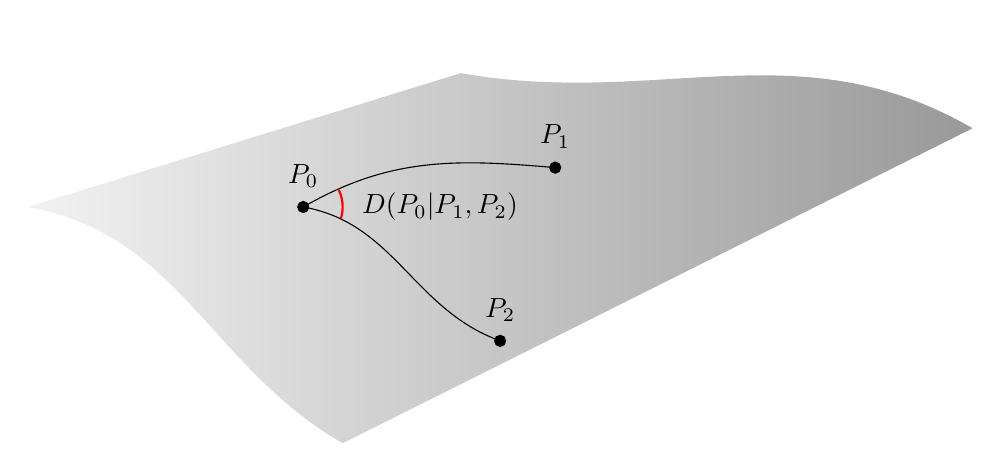
\begin{tikzpicture}
        % We draw the surface first
        \shade[left color=gray!10,right color=gray!80] 
        (0, 0) to[out=-10,in=150] (4  , -3) --
        (12,1) to[out=150,in=-10] (5.5,1.7) -- cycle;

        % Node corresponding to P_0
        \node at ($(3.5, 0)$) (P_0) {};
        \draw[fill] (P_0) circle (2pt);
        \node[above = of P_0, yshift = -1cm] {$P_0$};
        
        % Node corresponding to P_1
        \node at ($(6.7, 0.5)$) (P_1) {};
        \draw[fill] (P_1) circle (2pt);
        \node[above = of P_1, yshift = -1cm] {$P_1$};
        
        % Node corresponding to P_2
        \node at ($(6, -1.7)$) (P_2) {};
        \draw[fill] (P_2) circle (2pt);
        \node[above = of P_2, yshift = -1cm] {$P_2$};

        % Curved line
        \draw (P_0.center) to [out=30,in=175] (P_1.center);
        \draw (P_0.center) to [out=-10,in=160] (P_2.center);

        % Arc
        \draw [red,thick,domain=-17:26]
        plot ({3.5 + 0.5 * cos(\x)}, {0.5 * sin(\x)}) ;
        
        \node[right = of P_0, xshift = -0.5cm]
        {$D(P_0 |P_1, P_2)$};
    \end{tikzpicture}
    }
    \caption{The codivergence between $P_1$ and $P_2$ at $P_0$ measures the position of $P_1$ and $P_2$ relative to $P_0.$}
    \label{fig:codiv}
\end{figure}

\medskip

For the application to statistics, $E$ is taken as the space of all finite signed measures on a measurable space $(\Ac, \Bc)$, and $\Xc$ is the space of all probability measures on a measurable space $(\Ac, \Bc)$.
A visual representation of such a codivergence is provided in Figure~\ref{fig:codiv} below.

\medskip

In a next step, we characterize the tangent spaces of a codivergence for $\Xc$ the space of probability measures. Given a probability measure $P_0 \in \Xc,$ we say that a function $h: \Xc \to \Rb$ is $P_0$-essentially bounded by a constant $C > 0$ if $P_0(\{x \in \Ac: |h(x)| \leq C \}) = 1$ and define $\EssSup_{P_0}|h| := \inf\{C > 0: \,
|h| \text{ is } P_0\text{-essentially bounded by } C \}.$ We will show that
\begin{align*}
    \Mc_{P_0} := \left\{ \mu \in E: \, 
    \mu \ll P_0, \,
    \int d\mu = 0, \,
    \EssSup_{P_0}\Big|\frac{d\mu}{dP_0}\Big| < + \infty
    \right\}
\end{align*}
is the largest tangent space that any codivergence on $\Xc$ can have at $P_0$. The rationale is that $P_0+t\mu$ is otherwise not a probability measure. Indeed if $\mu \in \Mc_{P_0}$ has a density $h$ with respect to $P_0$, then the $P_0$-density $1 + t h$ is non-negative for given $t>0$ if and only if $h$ is larger than $-1/t$. Conversely, the density $1 - t h$ is non-negative for given $t <0$ if and only if $h$ is smaller than $1/t$.
This gives a link between a bound on $h = d\mu/dP_0$ and the non-negativity of the probability measure $P_0 + t \mu.$


\begin{prop}
    For any codivergence $D$ on the space of probability measures $\Xc$, the tangent space of $D$ at any probability measure $P_0 \in \Xc$ must be included in $\Mc_{P_0}$.
    Furthermore, every $\mu \in \Mc_{P_0}$ has a density $d\mu / dP_0$ with respect to $P_0$ such that
    $\EssSup_{P_0}|d\mu / dP_0|
    = 1 / a_*$
    with $a_* := \sup \{ a > 0:\, P_0 + t \mu \in \Xc \, \text{for all } t \in [-a , a]\} \in (0, +\infty]$ and the convention $1/+ \infty = 0$.
\label{prop:biggest_tangent_space}
\end{prop}

%{\color{red}
%Equivalently, for any $\mu \in \Mc_{P_0}$, the quantity $1 / \EssSup_{P_0}|d\mu / dP_0|$ is exactly the size of the largest interval $[-a_*, a_*]$ such that $\forall t \in [-a_*, a_*]$, $P_0 + t \mu$ is a probability measure.
%} 

\begin{proof}
    We begin by proving the first part of Proposition~\ref{prop:biggest_tangent_space}.
    Let $\mu$ be a finite signed measure belonging to the tangent space at $P_0$ of some codivergence $D$ on the space of probability measures $\Xc$.
    For $a > 0$, we write $\mu \in R(a)$ if and only if $P_0 + t \mu \in \Xc$ for all $-a\leq t\leq a.$
    Since $\mu$ belongs to the tangent space of $D$ at $P_0$, Definition~\ref{def:codiv}(iii) implies existence of an open neighborhood $T$ of $0$ such that for any $t \in T$, $P_0 + t \mu \in \Xc$. Therefore, there exists $a > 0$ with $\mu\in R(a)$.
    
    \medskip

    We now show that $\mu \in R(a),$ for some $a>0,$ implies $\mu \ll P_0$.
    By the Lebesgue decomposition theorem (see Theorem 4.3.2 in \cite{MR3098996}),
    $\mu$ can always be decomposed as $\mu = \mu_A + \mu_S$, where $\mu_A$ is a signed measure that is absolutely continuous with respect to $P_0$, $\mu_S$ is a signed measure that is singular with respect to $P_0$,
    and $\mu_A$ and $\mu_S$ are orthogonal.
    By the Jordan decomposition (cf. Corollary 4.1.6 in \cite{MR3098996}), we decompose the signed measure
    $\mu_S = \alpha_+ \mu_{S,+} - \alpha_- \mu_{S,-}$
    into its positive and negative part $\mu_{S,+}$ and $\mu_{S,-}$. These two measures are orthogonal and $\alpha_+, \alpha_- \geq 0.$
    Then, $P_0 + a \mu = P_0 + \, a \mu_A + a \alpha_+ \mu_{S,+} - a \alpha_- \mu_{S,-}$ can be a probability measure only if $\alpha_- = 0$. This is because we can find a set $U$ such that $P_0(U) = \mu_A(U) = \mu_{S,+}(U) = 0$ and $\mu_{S,-}(U) = 1$.
    Therefore $(P_0 + a \mu)(U)
    = - a \alpha_- \mu_{S,-}(U) = - a \alpha_- \leq 0$.
    In the same way, $P_0 - a \mu$ can be a probability measure only if $\alpha_+ = 0$.
    Therefore, if $\mu \in R(a)$ for some $a>0$, then $\alpha_+ = \alpha_- = 0$, and $\mu = \mu_A$ is absolutely continuous with respect to $P_0$.

    \medskip

    Let $h$ be the density of $\mu$ with respect to $P_0$.
    Then
    \begin{align*}
        \frac{d(P_0 + t \mu)}{dP_0}
        = 1 + t \frac{d\mu}{dP_0} = 1 + t h.
    \end{align*}
    Note that $P_0 + t \mu$ is a signed measure integrating to $1$ if and only if $\int d\mu = \int h \, dP_0 = 0$.

    \medskip
    
    We now show that, for any $a > 0$, $\mu \in R(a)$ implies $\EssSup_{P_0} |h| \leq 1/a$.
    If $\mu \in R(a)$, then for any
    $A \in \Bc,$ $(P_0 + a \mu)(A) \geq 0$
    and $(P_0 - a \mu)(A) \geq 0$.
    Let us define the sets $A_+ := \{ x \in \Ac: \, 1 + a h(x) \geq 0\}$ and $A_- := \{ x \in \Ac: \, 1 - a h(x) \geq 0\}$.
    Let $A^C$ denote the complement of a set $A$.
    We have $(P_0 + a \mu)(A_+^C) = \int_{A_+^C} 1 + a h(x) dP_X(x) \leq 0$ since this is the integral of a negative function.
    Therefore $P_0(A_+^C) = 0$ and then $P_0(A_+) = 1$.
    Similarly, $(P_0 + a \mu)(A_-^C) = \int_{A_-^C} 1 - a h(x) dP_X(x) \leq 0.$ Hence, $P_0(A_-^C) = 0$ and $P_0(A_-) = 1$.

    Therefore, $P_0(A_+ \cap A_-) = 1$.
    This means that for $P_0$-almost every $x \in \Ac$, $1 + a h(x) \geq 0$ and $1 - a h(x) \geq 0$.
    Therefore, for $P_0$-almost every $x \in \Ac$, $|h(x)| \leq 1/a$.
    Therefore, $h$ is $P_0$-essentially bounded by $C := 1/a$.
    We have finally shown that $\mu\in R(a)$ implies $\EssSup_{P_0} |h| \leq 1/a$ and $\mu \in \Mc_{P_0}$, proving the first part of Proposition~\ref{prop:biggest_tangent_space}.

    \medskip

    Conversely, note that $\mu \in \Mc_{P_0}$ is a sufficient condition for $P_0 + t \mu$ to be a probability measure for all $t$ in a sufficiently small open neighborhood of $0$.

    \medskip
    
    We now show the second part of Proposition~\ref{prop:biggest_tangent_space}.
    Remember that $a_* := \sup \{ a > 0: \, \mu \in R(a) \} \in (0, + \infty]$.
    Let $(a_n)_{n \in \NN}$ be an increasing sequence of real numbers strictly smaller than $a_*$ and converging to $a_*$.
    For every positive integer $n$, we have $\mu \in R(a_n)$.
    Therefore, by the previous reasoning, $\EssSup_{P_0} |h| \leq 1/a_n$, meaning that $P_0(\{ x \in \Ac: \, |h(x)| \leq 1/a_n \}) = 1$.
    By a union bound, we obtain $P_0( \cap_{n \geq 0} \{ x \in \Ac: \, |h(x)| \leq 1/a_n \}) = 1$.
    Therefore $P_0( \{ x \in \Ac: \, |h(x)| \leq 1/a_* \}) = 1$, and by definition $\EssSup_{P_0}|h| \leq 1/ a_*$.

    We now show the reverse version of this inequality. Let $C > \EssSup_{P_0}|h|$.
    Then $P_0(\{x \in \Ac: \, |h(x)| \leq C\} = 1$.
    Hence, for any $t \in [-1/C, 1/C]$, and for $P_0$-almost every $x$, $-1 \leq t h(x) \leq 1$.
    Consequently, for any $t \in [-1/C, 1/C]$, and for $P_0$-almost every $x$,
    $1 + t h(x) \geq 0$ and $1 - t h(x) \geq 0$. For any $t \in [-1/C, 1/C]$, $P_0 + t \mu$ is a finite signed measure with a density that is non-negative $P_0$-almost everywhere and integrates to $1$.
    These are sufficient conditions for $P_0 + t \mu$ to be a probability measure on $\Ac$,
    % meaning that $\forall t \in [-1/C, 1/C]$, $P_0 + t \mu \in \Xc$.
    proving $\mu \in R(1/C)$.
    Therefore, $1/C \leq a_*$ and thus $1/a_* \leq C$. This holds for any $C > 0$ such that $C > \EssSup_{P_0}|h|$, proving that $1/a_* \leq \EssSup_{P_0}|h|$.
    Together with the inequality $\EssSup_{P_0}|h| \leq 1/ a_*$, the claim $1/a_* = \EssSup_{P_0}|h|$ follows.
\end{proof}



We define the $\chi^2$-codivergence and the Hellinger codivergence between three probability measures $P_0, P_1, P_2$ by
\begin{align*}
    \chi^2(P_0 | P_1, P_2) :=
    \begin{cases} \displaystyle
    \int \frac{dP_1}{dP_0} dP_2 - 1
    = \int \frac{p_1 p_2}{p_0} d\nu - 1,
    & \text{if }
    P_1 \ll P_0 \text{ and } P_2 \ll P_0, \\
    + \infty, & \text{else,}
    \end{cases}
\end{align*}
and 
\begin{align*}
    \rho(P_0 | P_1, P_2) :=
    \begin{cases} \displaystyle
    \dfrac {\int \sqrt{p_1 p_2}  \, d\nu}{
    \int \sqrt{p_1 p_0} \, d\nu 
    \int \sqrt{p_2 p_0} \, d\nu} 
    - 1,
    & \text{ if }
    \int \sqrt{p_1 p_0} \, d\nu
    \int \sqrt{p_2 p_0} \, d\nu > 0, \\
    + \infty, & \text{else,}
    \end{cases}
\end{align*}
where $\nu$ is a measure dominating $P_0, P_1, P_2$, for example $\nu = (P_0 + P_1 + P_2)/3$, and $p_0, p_1, p_2$ are respectively their $\nu$-densities. It can be seen from the definitions that both codivergences are independent of the choice of the dominating measure $\nu$. The condition for finiteness of the Hellinger codivergence is much weaker than the condition for finiteness of the $\chi^2$-codivergence as it is only required that the support of $p_0$ intersects with non-zero $\nu$-mass the support of $p_1$ and the support of $p_2$.

\medskip


The $\chi^2$-divergence is defined as $\chi^2(P,Q) := \int (dP/dQ-1)^2 dQ= \int (dP/dQ)^2 dQ-1$, if $P$ is dominated by $Q$ and $+\infty$ otherwise. Therefore, the $\chi^2$-codivergence $\chi^2(P_0 | P_1, P_1)$
coincides with the usual $\chi^2$-divergence $\chi^2(P_1, P_0)$ for any $P_0$ and $P_1$. On the contrary, there is no clear link between the Hellinger codivergence and the usual squared Hellinger distance $H(P,Q)^2 := \tfrac12 \int (\sqrt{P}-\sqrt{Q})^2=1-\int \sqrt{PQ}.$ We now compare the local behavior of $\rho$ and $\chi^2$.

\newpage

\begin{prop}

\begin{itemize}
    \item[(i)] For any probability measures $P_0, P_1 \in \Xc$, we have $\rho(P_0 | P_1, P_1) \leq \chi^2(P_0 | P_1, P_1)$,
    
    \item[(ii)] the $\chi^2$-codivergence and the Hellinger codivergence are codivergences in the sense of Definition \ref{def:codiv} with tangent spaces $\Mc_{P_0}$ and respective bilinear maps $\langle \mu, \wt \mu \rangle_{P_0}$ for the $\chi^2$-codivergence and $\langle \mu, \wt \mu \rangle_{P_0} / 4$ for the Hellinger codivergence, where
    \begin{align*}
        \langle \mu, \wt \mu \rangle_{P_0}
        := \int \frac{d \mu}{dP_0} d\wt \mu
        = \int h g \, dP_0,
        % = \int \frac{h g}{p_0} d\nu,
        % \quad \text{where} \ h = \frac{d\mu}{d\nu} \ \text{and} \ g = \frac{d\wt \mu}{d\nu},
        \quad \text{with} \ h = \frac{d\mu}{dP_0} \ \text{and} \ g = \frac{d\wt \mu}{dP_0}.
    \end{align*}

    \item[(iii)] if $\nu$ dominates $P_0$, the bilinear map can be written as
    $\displaystyle \langle \mu, \wt \mu \rangle_{P_0}
    = \int h g/p_0 \, d\nu$,
    for the densities $h = d\mu / d\nu$, $g = d\wt \mu / d\nu$
    and $p_0 = dP_0/d\nu$.
\end{itemize}

\label{prop:codiv}
\end{prop}


Since the bilinear forms coincide up to a factor $1/4$, locally, the $\chi^2$-codivergence and the Hellinger codivergence define the same structure. This scalar product is the nonparametric Fisher information metric as considered in \cite{holbrook2017nonparametric,srivastava2007riemannian,srivastava2016functional}.

\begin{proof}[Proof of Proposition~\ref{prop:codiv}]
    To see (i), observe that H\"older's inequality with $p=3/2$ and $q=3$ gives for any non-negative function $f,$ $1=\int p_1\leq (\int f^{3/2} p_1)^{2/3}(\int f^{-3}p_1)^{1/3}.$ The choice $f=(p_0/p_1)^{1/3}$ yields $1\leq (\int \sqrt{p_1p_0})^2 \int p_1^2/p_0.$
    Therefore $1 / (\int \sqrt{p_1p_0})^2 \leq \int p_1^2/p_0.$
    Subtracting one on each side of this expression yields the claim.
    
    \medskip

    We finally prove (ii).
    It is clear that both codivergences are symmetric, so the first part of Definition~\ref{def:codiv} is satisfied.
    The second part of Definition~\ref{def:codiv} is satisfied by the $\chi^2$-codivergence using the properties of the usual $\chi^2$ divergence.
    Moreover $\rho(P_0 | P_1, P_1) = 0$ if and only if
    $\int \sqrt{p_1 p_0} \, d\nu = 1$ if and only if $H^2(P_1, P_0) = 1$ if and only if $P_0 = P_1$.

    \medskip

    We now verify the third part of Definition~\ref{def:codiv}.
    Let $\mu, \wt \mu \in \Mc_{P_0}$. Then
    \begin{align*}
        \frac{d(P_0 + t \mu)}{dP_0}
        = 1 + t \frac{d\mu}{dP_0} = 1 + t h,
    \end{align*}
    is square-integrable with respect to $P_0$ for any real number $t$.
    % Therefore $\chi^2(P_0 | P_0 + t \mu, P_0 + s \wt \mu)$ is finite for any choice of $s, t \in \Rb$, and $(1 + t h) (1 + s g)$ is $P_0$-integrable.
    We can write
    \begin{align*}
        \chi^2(P_0 | P_0 + t \mu, P_0 + s \wt \mu) 
        = \int (1 + t h) (1 + s g) \, dP_0 - 1
        = \int (t h + s g + t s hg) \, dP_0
        = t s \int h g \, dP_0,
    \end{align*}
    as claimed, since $\int h \, dP_0 = \int g \, dP_0 = 0$.
    % (otherwise $P_0 + t \mu$ and $P_0 + s \wt\mu$ could not integrate to one).
    We now consider the case of the Hellinger codivergence. Taylor expansion $\sqrt{1+x} = 1 + x/2 - x^2/8 + o(x^2)$ yields $\int \sqrt{1 + t h} \, dP_0
    = 1 - t^2  \int h^2 dP_0/8 + o(t^2)$
    and
    \begin{align*}
        \int \sqrt{(1 + t h) (1 + s g)} \, dP_0
        &= \int \sqrt{1 + t h + s g + t s g h} \, dP_0 \\
        %
        &= \int \bigg( 1 + \frac{t h + s g + t s g h}{2}
        - \frac{(t h + s g + t s g h)^2}{8} \bigg) \, dP_0 \\
        %
        &= \int \bigg( 1 + \frac{t h + s g + t s g h}{2}
        - \frac{t^2 h^2 + s^2 g^2 + 2 t h s g + o(t^2 + s^2)}{8} \bigg) \, dP_0 \\
        %
        &= 1 + t s \int \frac{h g}{4} dP_0
        - t^2 \int \frac{h^2}{8} dP_0
        - s^2 \int \frac{g^2}{8} dP_0
        + o(t^2 + s^2),
    \end{align*}
    where all integrals are finite since the integrands are bounded.
    Combining these expansions with the Taylor expansion
    $1/(1-x) = 1 + O(x)$ for $|x|\leq 1/2,$ we get for all sufficiently small real numbers $a,b,c,$
    \begin{align*}
        \frac{1-a+b}{1-a+c}-1= \frac{b-c}{1-a+c}=(b-c)\Big(1+O(a-c)\Big).
    \end{align*}
    Thus with $a=(t^2\int h^2 dP_0+s^2\int g^2 dP_0)/8,$ $b=ts \int hg dP_0/4+o(t^2+s^2)$ and $c=o(t^2+s^2),$
    \begin{align*}
        \rho(P_0 | P_0 + t \mu, P_0 + s \wt \mu)
        &:= \dfrac {\int
        \sqrt{(1 + t h) (1 + s g)}  \, dP_0}{
        \int \sqrt{1 + t h} \, dP_0
        \int \sqrt{1 + s g} \, dP_0} 
        - 1 \\
        %
        &= \frac{1-a+b}{1-a+c}-1 \\
        &= (b-c)\Big(1+O(a-c)\Big)\\
        &= t s \int \frac{h g}{4} dP_0
        + o(t^2 + s^2),
    \end{align*}
    as claimed.
\end{proof}

A more general expansion is possible for the Hellinger codivergence. Assume that $P_0$ is dominated by some positive measure $\nu$. Define $\support(\mu) := \{ x \in \Ac: d\mu/d\nu(x) \neq 0\}$ for any signed measure $\mu$ dominated by $\nu.$ If $\mu_1$ and $\mu_2$ are signed measures dominated by $\nu$ such that (i) $\support(\mu_i) \cap \support(P_0)$ has a positive $\nu$-measure, and (ii) their densities $h_i$ are positive on $\support(\mu_i) \backslash \support(P_0)$, then
\begin{align}
    \rho(P_0 &| P_0 + t \mu_1, P_0 + s \mu_2)
    = \sqrt{t s} \int_{\support(P_0)^C} \sqrt{h_1 h_2} \, d\nu
    + t s \int_{\support(P_0)} \frac{h_1 h_2}{2 p_0} \, d\nu
    + o(t^2 + s^2).
    \label{eq:general_expansion_rho}
\end{align}
If compared to Definition~\ref{def:codiv} (iii) there is thus an additional term for probability measures that have mass outside of the support of $P_0$. Consequently, this expansion cannot be linked to one local bilinear form and the mapping $(t, s) \in \Rb_+^2 \mapsto \rho(P_0 | P_0 + t \mu_1, P_0 + s \mu_2)$ is not differentiable at $(0,0)$. This is in line with Proposition~\ref{prop:biggest_tangent_space}: for perturbations $\mu$ that do not belong to $\Mc_{P_0}$, the measures $P_0 + t \mu$ cannot be probability measures for all $t$ in any open neighborhood of $0$. %This explains why we need to assume $t > 0$ in Definition \ref{def:codiv}, and why the term $\sqrt{t}$ arises in Equation~\eqref{eq:general_expansion_rho}.}

\medskip

For a number of distributions, closed-form expressions for the $\chi^2$- and the Hellinger codivergences are reported in Table \ref{tab.1}. Derivations for these expressions are given in Section \ref{sec.explicit}. This section also contains expressions for the Gamma distribution that are not presented in the table to save space.
As mentioned before, these two codivergences quantify to which extent the measures $P_1$ and $P_2$ represent different directions around $P_0.$ The explicit formulas show this in terms of the parameters and reveal significant similarity between the $\chi^2$-codivergence and the Hellinger codivergence.
For the multivariate normal distribution, for instance, the $\chi^2$-codivergence and the Hellinger codivergence vanish if and only if the vectors $\theta_1-\theta_0$ and $\theta_2-\theta_0$ are orthogonal.

\medskip

\begin{table}[ht]
    \centering
    \renewcommand{\arraystretch}{1.5}
%     \resizebox{\textwidth}{!}{%
% % \begin{tabular}{m{3.2cm}|m{4.8cm}|m{5.5cm}}
% \begin{tabular}{c|c|c}
%     \text{distribution}
%     & $\chi^2(P_0,\dots,P_M)_{j,k}$ & $\rho(P_0 | P_1,\dots,P_M)_{j,k}$
%     \\ \hline
%     $P_j=\Nc(\theta_j, \sigma^2 I_d),$ 
% & \multirow{2}{*}{$\exp\Big(\dfrac{\langle \theta_j - \theta_0, \theta_k - \theta_0 \rangle}{\sigma^2}\Big) -1$ }
% & \multirow{2}{*}{$\exp\Big(\dfrac{\langle \theta_j - \theta_0, \theta_k - \theta_0 \rangle}{4\sigma^2}\Big) -1$} \\  
% $\theta_j \in \Rb^d,$ $I_d$ identity &&
%     \\ \hline
%     $P_j = \otimes_{\ell=1}^d \Pois(\lambda_{j\ell}),$ 
% & \multirow{2}{*}{$\exp\Big( \sum_{\ell=1}^d \dfrac{(\lambda_{j\ell}-\lambda_{0\ell})(\lambda_{k\ell}-\lambda_{0\ell})}{\lambda_{0\ell}}\Big)-1$}
% & ${\exp\Big( \sum_{\ell=1}^d \big(\sqrt{\lambda_{j\ell}}-\sqrt{\lambda_{0\ell}}\big)}$ \\ 
% $\lambda_{j\ell}>0$  & &
% $\qquad \times \big(\sqrt{\lambda_{k\ell}}-\sqrt{\lambda_{0\ell}}\big)\Big) -1$
%     \\  \hline
%     $P_j = \otimes_{\ell=1}^d \Exp(\beta_{j\ell}),$ &
% \multirow{2}{*}{$\prod_{\ell=1}^d
% \dfrac{ \beta_{j\ell} \beta_{k\ell}}
% {\beta_{0\ell} \big(\beta_{j\ell}+\beta_{k\ell}-\beta_{0\ell} \big)}
% - 1$}
% & \multirow{2}{*}{$\prod_{\ell=1}^d
% \dfrac {
% (\beta_{j\ell} + \beta_{0\ell}) (\beta_{k\ell} + \beta_{0\ell}) }
% {2 \beta_{0\ell} (\beta_{j\ell} + \beta_{k\ell}) }
% - 1$ }   
% \\ 
% $\beta_{j\ell}>0$& &
%     \\ \hline
%      \multirow{2}{*}{$P_j = \otimes_{\ell=1}^d \Ber(\theta_{j\ell}),$}
% & \multirow{3}{*}{$\prod_{\ell=1}^d
% \Big(\dfrac{
% (\theta_{j\ell} - \theta_{0\ell})
% (\theta_{k\ell} - \theta_{0\ell}) }
% {\theta_{0\ell}(1-\theta_{0\ell})} + 1 \Big) - 1$}
% &  
%  \multirow{2}{*}{$\prod_{\ell=1}^d \dfrac{r(\theta_{j\ell},\theta_{k\ell})}
% {r(\theta_{j\ell},\theta_{0\ell})r(\theta_{k\ell},\theta_{0\ell})}-1,$ with} \\
%  & & 
% \\
% $\theta_{j\ell}\in (0,1)$ & &  $r(\theta,\theta'):=\sqrt{\theta\theta'}+\sqrt{(1-\theta)(1-\theta')}$
% \\
% \end{tabular}
    \resizebox{\textwidth}{!}{%
% \begin{tabular}{m{3.2cm}|m{4.8cm}|m{5.5cm}}
\begin{tabular}{c|c|c}
    \text{distribution}
    & $\chi^2(P_0 | P_1, P_2)$ & $\rho(P_0 | P_1, P_2)$
    \\ \hline
    $P_j=\Nc(\theta_j, \sigma^2 I_d),$ 
    & \multirow{2}{*}{$\exp\Big(\dfrac{\langle \theta_1 - \theta_0, \theta_2 - \theta_0 \rangle}{\sigma^2}\Big) -1$ }
    & \multirow{2}{*}{$\exp\Big(\dfrac{\langle \theta_1 - \theta_0, \theta_2 - \theta_0 \rangle}{4\sigma^2}\Big) -1$} \\ 
    $\theta_j \in \Rb^d,$ $\sigma > 0$ &&
    \\ \hline
    %
    $P_j = \otimes_{\ell=1}^d \Pois(\lambda_{j\ell}),$ 
    & \multirow{2}{*}{$\exp\Big( \sum_{\ell=1}^d \dfrac{(\lambda_{1\ell}-\lambda_{0\ell})(\lambda_{2\ell}-\lambda_{0\ell})}{\lambda_{0\ell}}\Big)-1$}
    & ${\exp\Big( \sum_{\ell=1}^d \big(\sqrt{\lambda_{1\ell}}-\sqrt{\lambda_{0\ell}}\big)}$ \\
    $\lambda_{j\ell}>0$
    &  &
    $\qquad \times \big(\sqrt{\lambda_{2\ell}}-\sqrt{\lambda_{0\ell}}\big)\Big) -1$
    \\  \hline
    %
    $P_j = \otimes_{\ell=1}^d \Exp(\beta_{j\ell}),$
    & $\prod_{\ell=1}^d
    \dfrac{ \beta_{1\ell} \beta_{2\ell}}
    {\beta_{0\ell} \big(\beta_{1\ell}+\beta_{2\ell}-\beta_{0\ell} \big)}
    - 1,$
    & \multirow{2}{*}{$\prod_{\ell=1}^d
    \dfrac {
    (\beta_{1\ell} + \beta_{0\ell}) (\beta_{2\ell} + \beta_{0\ell}) }
    {2 \beta_{0\ell} (\beta_{1\ell} + \beta_{2\ell}) }
    - 1$ }   
    \\ 
    $\beta_{j\ell}>0$
    & if $\beta_{0\ell} < \beta_{1\ell} + \beta_{2\ell},$
    and $+\infty$ else
    &
    \\ \hline
    %
    \multirow{2}{*}{$P_j = \otimes_{\ell=1}^d \Ber(\theta_{j\ell}),$}
    & \multirow{3}{*}{$\prod_{\ell=1}^d
    \Big(\dfrac{
    (\theta_{1\ell} - \theta_{0\ell})
    (\theta_{2\ell} - \theta_{0\ell}) }
    {\theta_{0\ell}(1-\theta_{0\ell})} + 1 \Big) - 1$}
    &  
    \multirow{2}{*}{$\prod_{\ell=1}^d \dfrac{r(\theta_{1\ell},\theta_{2\ell})}
    {r(\theta_{1\ell},\theta_{0\ell})r(\theta_{2\ell},\theta_{0\ell})}-1,$ with} \\
    & & 
    \\
    $\theta_{j\ell}\in (0,1)$ & &  $r(\theta,\theta'):=\sqrt{\theta\theta'}+\sqrt{(1-\theta)(1-\theta')}$
    \\
\end{tabular}
}
\caption{Closed-form expressions for the $\chi^2$-codivergence and Hellinger codivergence for some parametric distributions. Proofs can be found in Section \ref{sec.explicit}.}
\vspace{0.5cm}
    \label{tab.1}
\end{table}



\section{Divergence matrices}
\label{sec:div_matrices}

\begin{defi}
    Let $M\geq 1.$ For a given codivergence $D( \cdot | \cdot, \cdot)$ on a space $\Xc \subset E$ and $u, v_1, \dots, v_M$ elements of $\Xc$, we define the divergence matrix $D(u | v_1, \dots, v_M)$ as the $M \times M$-matrix with $(j,k)$-th entry
    $D(u | v_1, \dots, v_M)_{j,k} := D(u | v_j, v_k)$, for $1 \leq j,k \leq M$.
\end{defi}

If $v_1, \dots, v_M$ are all in a neighborhood of $u$, the divergence matrix $D$ can be related to the Gram matrix of the bilinear form
$\langle \cdot, \cdot \rangle_{u}$.
Formally, for $\t = (t_1, \dots, t_M) \in \Rb^M$ such that for any $i = 1, \dots, M, \, u + t_i h_i \in \Xc$, we have
\begin{align*}
    D(u | u + t_1 h_1, \dots, u + t_M h_M)
    % = [t_i t_j \langle h_i, h_j \rangle_{u}]_{1 \leq i,j \leq M} + o(\|\mathbf{t}^2\|)
    = \t \Gb_{u}  \t^\top + o(\|\mathbf{t}\|^2),
\end{align*}
with Gram matrix $\Gb_{u}
:= (\langle h_i, h_j \rangle_{u})_{1 \leq i,j \leq M}$.

\medskip

As in the previous section,
the $\chi^2$-divergence matrix $\chi^2(P_0 | P_1, \dots, P_M)$
and the Hellinger affinity matrix $\rho(P_0 | P_1, \dots, P_M)$ are respectively defined
as the $M\times M$ matrices with $(j,k)$-th entry
\begin{align*}
    &\chi^2(P_0 | P_1, \dots, P_M)_{j,k}
    := \int \frac{dP_j}{dP_0} dP_k - 1
    \text{, and,} \\
    %
    &\rho(P_0 | P_1, \dots, P_M)_{j,k}
    := \frac {\int \sqrt{p_j p_k}  \, d\nu}
    {\int \sqrt{p_j p_0  }\, d\nu  \int \sqrt{p_k p_0} \, d\nu} -1,
    % , \quad j,k=1,\dots, M.
\end{align*}
for $1 \leq j, k \leq M$. They correspond to the divergence matrices of the $\chi^2$-codivergence and the Hellinger codivergence.
Therefore, by Proposition~\ref{prop:codiv},
the local Gram matrix of $\chi^2$ at a distribution $P_0$ is
$\Gb_{P_0} := \big[\int \frac{h_i h_j}{p_0} d\nu \big]_{1 \leq i,j \leq M},$
and the local Gram matrix of $\rho$ is $\Gb_{P_0} / 4$.
We give now a few properties of these matrices.
\begin{prop}
\label{prop:div_matrices}
\begin{itemize}
    \item[(i)] The $\chi^2$-divergence matrix and the Hellinger affinity matrix are both symmetric and positive semi-definite.

    \item[(ii)] For any vector $\v=(v_1,\dots,v_M)^\top \in \Rb^M,$ we have the identity 
    \begin{align}
        \v^\top \chi^2(P_0 | P_1, \dots, P_M) \v
        = \int \Big(\sum_{j=1}^M \Big(\frac{dP_j}{dP_0}-1\Big) v_j \Big)^2 dP_0,
        \label{eq.chi2_int_representation}
    \end{align}
    and therefore
    $\v^\top \chi^2(P_0 | P_1, \dots, P_M) \v = \chi^2(\sum_{j=1}^M v_j P_j, P_0),$ 
    where $\sum_{j=1}^M v_j P_j$ is the mixture (signed) measure of $P_1, \dots, P_M$.
    
    \item[(iii)] $\chi^2(P_0 | P_1, \dots, P_M) = \Cov_{P_0}(\Z)$, where $\Z := (dP_1/dP_0(X), \dots, dP_M/dP_0(X))^\top$ is the random vector containing the likelihood ratios of the $M$ measures with $X \sim P_0$.
    
    
    \item[(iv)] $\Rank(\chi^2(P_0 | P_1, \dots, P_M)) = \Rank(dP_1/dP_0, \dots, dP_M/dP_0)$, where linear independence is considered $P_0$-almost everywhere.

    \item[(v)] For any vector $v=(v_1,\dots,v_M)^\top \in \Rb^M,$ we have the identity 
    \begin{align}
        \v^\top \rho(P_0 | P_1,\dots,P_M) \v
        = \int \bigg( \sum_{j=1}^M \Big(\frac{\sqrt{p_j}}{\int \sqrt{p_j p_0}\, d\nu}-\sqrt{p_0} \Big) v_j \bigg)^2\, d\nu.
        \label{eq.Hell_aff_pos_def}
    \end{align}
    
    \item[(vi)] $\Rank(\rho(P_0 | P_1, \dots, P_M)) = \Rank(\sqrt{dP_1/dP_0}, \dots, \sqrt{dP_M/dP_0})$, where linear independence is considered $P_0$-almost everywhere.
    
    \item[(vii)] Furthermore, if $P_1, \dots, P_M$ are all dominated by $P_0$, then 
    \begin{align*}
        \v^\top \rho(P_0 | P_1,\dots,P_M) \v
        = E_{P_0} \left[ \left(
        \sum_{j=1}^M \frac{\sqrt{dP_j/dP_0}
        - E_{P_0} \big[ \sqrt{dP_j/dP_0} \, \big]}{
        E_{P_0} \big[ \sqrt{dP_j/dP_0} \, \big]} v_j
        \right)^2 \right].
    \end{align*}
    Therefore $\rho(P_0 | P_1,\dots,P_M)
    = \Diag \big(E_{P_0}[\sqrt{\Z}] \big)^{-1}
    \Cov_{P_0} \big(\sqrt{\Z} \big)
    \Diag \big(E_{P_0}[\sqrt{\Z}] \big)^{-1},$
    where $\Diag(\a)$ denotes the diagonal matrix with diagonal equal to the vector $\a$ and $\sqrt{\Z}$ is defined as the random vector $(\sqrt{dP_1/dP_0(X)}, \dots, \sqrt{dP_M/dP_0(X)})^\top$, that is, the componentwise square-root of $\Z$.
    
\end{itemize}
\end{prop}

We remark that the representations given in (iii) and (vii) can also provide a direct way of recovering the local Gram matrix associated to the nonparametric Fisher information metric. In this case, the Taylor expansion would be applied to the density ratio $\Z$.

\begin{proof}
(i) is a consequence of (ii) and (v).
(ii) and (v) can be shown by expanding the squares on the right-hand side of Equation~\eqref{eq.chi2_int_representation} and Equation~\eqref{eq.Hell_aff_pos_def}.
(iii) is a consequence of (ii) and the fact that the expectation of each component of $\Z$ under $P_0$ is $1$.
(vii) is a consequence of the representation (v) and the domination assumption.

We now prove (iv).
Let $r := \Rank(\chi^2(P_0 | P_1, \dots, P_M))$.
Applying (iii) and then Lemma~\ref{lemma:rank_CovZ}, we obtain that $r = \Rank(\Cov_{P_0}(\Z)) = \Rank(Z_1, \dots, Z_M)$.
By Lemma~\ref{lemma:rank_max_lincombin}, $r$ is the highest integer such that there exists $i_1, \dots, i_r \in \{1, \dots, M\}$ with $(Z_{i_1}, \dots, Z_{i_r})$ linearly independent random variables $P_0$-almost surely.

Using the fact that
$\Z := (dP_1/dP_0(X), \dots, dP_M/dP_0(X))^\top$ and $X \sim P_0$, the random variables $\{Z_{i_1}, \dots, Z_{i_r}\}$ are linearly independent $P_0$-almost surely if and only if
$P_0(\sum_{j=1}^r a_j dP_{i_j}/dP_0(X) = 0) = 1$ implies $a_1=\ldots=a_r=0$.
This is the case if and only if 
the functions $\{dP_{i_1}/dP_0, \dots, dP_{i_r}/dP_0\}$ are linearly independent $P_0$-almost everywhere, proving $\Rank(Z_{i_1}, \dots, Z_{i_r})
= \Rank(dP_{i_1}/dP_0, \dots, dP_{i_r}/dP_0)$.

\medskip

We now show (vi). We prove in a first step that $\Rank(\rho(P_0 | P_1, \dots, P_M)) = M$ if and only if all the $M$ functions $\sqrt{dP_1/dP_0}, \dots, \sqrt{dP_M/dP_0}$ are linearly independent $P_0$-almost everywhere.
The matrix is singular if and only if there exists a non-null vector $v$ such that
$\sum_{j=1}^M \frac{v_j \sqrt{p_j}}{\int \sqrt{p_j p_0}\, d\nu}
= \sum_{j=1}^M v_j \sqrt{p_0}$ $\nu$-almost everywhere.
This is the case if and only if there are numbers $w_0,\dots,w_M,$ that are not all equal to zero, satisfying $\sum_{j=0}^M w_j\sqrt{p_j}=0,$ $\nu$-almost everywhere. To verify the more difficult reverse direction of this equivalence, it is enough to observe that $\sum_{j=0}^M w_j\sqrt{p_j}=0$ implies $w_0=- \sum_{j=1}^M w_j \int \sqrt{p_j p_0}\, d\nu$ and thus, taking $v_j=w_j \int \sqrt{p_j p_0}\, d\nu$ yields $\sum_{j=1}^M \frac{v_j \sqrt{p_j}}{\int \sqrt{p_j p_0}\, d\nu}
= \sum_{j=1}^M v_j \sqrt{p_0}.$

\medskip

We now show the general case of (vi). Let $r$ be an integer in $\{1, \dots, M\}$. Note that
$$r = \Rank(\rho(P_0 | P_1, \dots, P_M))$$
% if and only if
% $$\Rank(\rho(P_0 | P_1, \dots, P_M)) < r+1 \text{ and }
% \Rank(\rho(P_0 | P_1, \dots, P_M)) \geq r$$
if and only if (by Lemma \ref{lemma:rank_principal_minors})
$$\begin{array}{c}
\rho(P_0 | P_1, \dots, P_M)
\text{ has an invertible principal submatrix of size } r \\
\text{ and all principal submatrix of size } r+1 
\text{ of } \rho(P_0 | P_1, \dots, P_M) 
\text{ are singular}
\end{array}
$$
if and only if (using the fact that the principal submatrices of $\rho(P_0 | P_1, \dots, P_M)$ of size $k$ are exactly the matrices of the form $\rho(P_0 | P_{i_1}, \dots, P_{i_k})$ for some $i_1, \dots, i_k \in \{1, \dots M\}$)
\begin{align*}
    r = \max_{} \{k=1, \dots, M: \,
    \exists i_1, \dots, i_k \in \{1, \dots, M\}, \,
    \rho(P_0 | P_{i_1}, \dots, P_{i_k}) \text{ is invertible} \}
\end{align*}
% is the maximum integer $k$ such that there exist $k$ probability distributions $P_{i_1}, \dots, P_{i_r}$ such that $\rho(P_0 | P_{i_1}, \dots, P_{i_r})$ is invertible
if and only if (using the case of full rank that was proved before)
\begin{align*}
    r = \max_{} \{k=1, \dots, M: \,
    \exists i_1, \dots, i_k \in \{1, \dots, M\}, \,
    \sqrt{dP_{i_1}/dP_0}, \dots, \sqrt{dP_{i_r}/dP_0}
    \text{ are linearly independent} \}
\end{align*}
% $r$ is the maximum integer $k$ such that there exist $k$ functions $\sqrt{dP_{i_1}/dP_0}, \dots, \sqrt{dP_{i_r}/dP_0}$ that are linearly independent $P_0$-almost everywhere
if and only if 
$r = \Rank(\sqrt{dP_1/dP_0}, \dots, \sqrt{dP_M/dP_0}).$

% 
% We finally show (viii). By the representations (iii) and (vii), and remembering that $E_{P_0}[Z_i] = 1$ for any $i=1, \dots, M$ we have
% \begin{align*}
%     \v^\top \big(\chi^2 - \rho \big) \v
%     &= \v^\top \Cov_{P_0}[\Z] \v
%     - E_{P_0} \left[ \left(
%     \sum_{j=1}^M \frac{\sqrt{Z_j}
%     - E_{P_0} \big[ \sqrt{Z_j} \, \big]}{
%     E_{P_0} \big[ \sqrt{Z_j} \, \big]} v_j \right)^2 \right] \\
%     %
%     &= \sum_{i, j=1}^M E_{P_0}
%     \left[ (Z_i Z_j - 1) - \frac{\sqrt{Z_i Z_j}
%     - E_{P_0} \big[ \sqrt{Z_i} \, \big]
%     E_{P_0} \big[ \sqrt{Z_j} \, \big]}{
%     E_{P_0} \big[ \sqrt{Z_i} \, \big]
%     E_{P_0} \big[ \sqrt{Z_j} \, \big]} \right] v_i v_j \\
%     %
%     &= \sum_{i, j=1}^M E_{P_0}
%     \left[ Z_i Z_j - \frac{\sqrt{Z_i Z_j}}{
%     E_{P_0} \big[ \sqrt{Z_i} \, \big]
%     E_{P_0} \big[ \sqrt{Z_j} \, \big]} \right] v_i v_j \\
%     %
%     &= E_{P_0}[\v^\top \Z \Z^\top \v]
%     - E_{P_0} \left[\v^\top
%     \Big(\sqrt{\Z} \oslash E_{P_0} \big[ \sqrt{\Z} \, \big] \Big)
%     \Big(\sqrt{\Z} \oslash E_{P_0} \big[ \sqrt{\Z} \, \big] \Big)^\top \v \right]
% \end{align*}
% 
% 
\end{proof}



% \newpage

\section{Data processing inequality for the \texorpdfstring{$\chi^2$}{chi2}-divergence matrix}
\label{sec:data_processing}

In a parametric statistical model $(Q_\theta)_{\theta \in \Theta}$, it is assumed that the statistician observes a random variable $X$ following one of the distributions $Q_\theta$ for some $\theta \in \Theta$. If we transform $X$ to obtain a new variable $Y$, then $Y$ follows the distribution $P_\theta := K Q_\theta$ for some Markov kernel $K$. When $\theta$ is unknown but the Markov kernel $K$ is known and independent of $\theta$, this means that the new statistical model is $(P_\theta := K Q_\theta, \, \theta \in \Theta)$.
As in the usual case for the $\chi^2$-divergence, it is natural to think that such a transformation cannot increase the quantity of information present in the model.
In our more general framework, such an inequality still holds and is presented in the following data processing inequality.
\begin{thm}[Data processing / entropy contraction]\label{thm.data_processing}
    If $K$ is a Markov kernel and $Q_0,\dots,Q_M$ are probability measures such that $Q_0$ dominates $Q_1,\dots,Q_M,$ then,
    \begin{align*}
        \chi^2\big(K Q_0,\dots, KQ_M\big) 
        \leq \chi^2\big(Q_0,\dots, Q_M\big),
    \end{align*}
    where $\leq$ denotes the partial order on the set of positive semi-definite matrices.
\end{thm}
In particular, the $\chi^2$-divergence matrix is invariant under invertible transformations.
The rest of this section is devoted to the proof of Theorem \ref{thm.data_processing}.
First, we generalize the well-known data-processing inequality for the $\chi^2$-divergence to the case where one measure is a finite signed measure and then we will use Equation~\eqref{eq.chi2_int_representation}.

\medskip

Let $\mu$ be a finite signed measure and $P$ be a probability measure defined on the same measurable space $(\Omega, \mathcal{A})$. We define the $\chi^2$-divergence of $\mu$ and $P$ by
\begin{align}
    \chi^2(\mu,P) := \begin{cases}
    \displaystyle \int \Big( \frac{d\mu}{dP} - \mu(\Omega)\Big)^2 \, dP,
    & \text{ if } \mu\ll P, \\
    + \infty & \text{ else.}
    \end{cases} 
    \label{eq.chi_divergence_signed_measure}
\end{align}
Here, $d\mu/dP$ denotes the Radon-Nikodym derivative of the signed measured $\mu$ with respect to $P$ (defined e.g. in Theorem 4.2.4 in \cite{MR3098996}).
This definition of $\chi^2(\mu,P)$ generalizes the case where $\mu$ is a probability measure. This quantity $\chi^2(\mu,P)$ can be computed from the usual $\chi^2$-divergence between probability measures by the following relationship
\begin{lemma}
    Assume that $\mu \ll P$.
    Let $\mu=\alpha_+\mu_+-\alpha_-\mu_-$ be the Jordan decomposition (cf. Corollary 4.1.6 in \cite{MR3098996}) of $\mu$ with $\alpha_+, \alpha_- \geq 0$ and $\mu_+,$ $\mu_-$ orthogonal probability measures.
    Then 
    $$\chi^2(\mu,P) = \alpha_+^2 \chi^2\big(\mu_+,P\big)
    + \alpha_-^2 \chi^2 \big(\mu_- , P\big) + 2\alpha_+ \alpha_-.$$
    \label{lemma:chi2_signed_measure}
\end{lemma}
\begin{proof}
    Observe that $\displaystyle \alpha_+^2 \chi^2\big(\mu_+,P\big)
    +\alpha_-^2 \chi^2\big(\mu_-,P\big)
    +2\alpha_+\alpha_- 
    =\int \Big(\alpha_+\Big(\frac{d\mu_+}{dP}-1\Big)-\alpha_-\Big(\frac{d\mu_-}{dP}-1\Big)\Big)^2 \, dP
    = \int \Big(\frac{d\mu}{dP}-\mu(\Omega)\Big)^2 \, dP
    =\chi^2(\mu,P).$
\end{proof}

\medskip

\begin{lemma}
    If $\mu$ is a finite signed measure, $P$ is a probability measure and both measures are defined on the same measurable space, then, for any Markov kernel $K,$ the data-processing inequality
    \begin{align*}
        \chi^2(K\mu,KP)
        \leq \chi^2(\mu,P)
    \end{align*}
    holds.
    \label{lem.data_processing_signes_measure}
\end{lemma}

\begin{proof}
We can assume that $\mu \ll P,$ since otherwise the right-hand side of the inequality is $+\infty$ and the result holds. In particular, $\mu \ll \nu$ for a positive measure $\nu$ implies that $K\mu \ll K\nu.$ Indeed, if $K\nu(A)=0$ for a given measurable set $A$, then, $\int K(A,x) \, d\nu(x)=0,$ implying $K(A,\cdot)=0$ $\nu$-almost everywhere. Since $\mu\ll \nu,$ the equality also holds $\mu$-almost everywhere and so $K\mu(A)=\int K(A,x)d\mu(x)=0,$ proving $K\mu \ll K\nu.$ By the Jordan decomposition (cf. Corollary 4.1.6 in \cite{MR3098996}), there exist orthogonal probability measures $\mu_+,$ $\mu_-$ and non-negative real numbers $\alpha_+,\alpha_-,$ such that $\mu=\alpha_+\mu_+-\alpha_-\mu_-$ and $\mu(
\Omega)=\alpha_+-\alpha_-.$ Thus, $K\mu=\alpha_+K\mu_+-\alpha_-K\mu_-.$ Observe that 
\begin{align*}
    \int \Big(\frac{dK\mu_+}{dKP}-1\Big)\Big(\frac{dK\mu_-}{dKP}-1\Big) \, dKP
    &= \int \bigg(  \frac{dK\mu_+}{dKP} \frac{dK\mu_-}{dKP}
    - \frac{dK\mu_-}{dKP}
    - \frac{dK\mu_+}{dKP}
    + 1 \bigg) \, dKP \\ 
    &= \int \frac{dK\mu_+}{dKP} \frac{dK\mu_-}{dKP} \, dKP-1
    \geq -1.
\end{align*}
Because $\mu_+$ and $\mu_-$ are orthogonal, we similarly find that 
\begin{align*}
    \int \Big(\frac{d\mu_+}{dP}-1\Big)\Big(\frac{d\mu_-}{dP}-1\Big) \, dP =-1.
\end{align*}
Using the data-processing inequality for the $\chi^2$ divergence of probability measures twice, $K\mu=\alpha_+K\mu_+-\alpha_-K\mu_-$ and $\mu(\Omega)=\alpha_+-\alpha_-,$ we get
\begingroup \allowdisplaybreaks
\begin{align*}
    \chi^2(K\mu, KP)
    &=
    \int \Big(\frac{dK\mu}{dKP}-\mu(\Omega)\Big)^2 \, dKP \\
    &= 
    \int \Big(\alpha_+\Big(\frac{dK\mu_+}{dKP}-1\Big)-\alpha_-\Big(\frac{dK\mu_-}{dKP}-1\Big)\Big)^2 \, dKP \\
    &= \alpha_+^2 \chi^2\big(K\mu_+,KP\big)
    +\alpha_-^2 \chi^2\big(K\mu_-,KP\big)
    - 2\alpha_+\alpha_-\int \Big(\frac{dK\mu_+}{dKP}-1\Big)\Big(\frac{dK\mu_-}{dKP}-1\Big) \, dKP \\
    &\leq \alpha_+^2 \chi^2\big(\mu_+,P\big)
    +\alpha_-^2 \chi^2\big(\mu_-,P\big)
    +2\alpha_+\alpha_- =\chi^2(\mu,P),
\end{align*}
\endgroup
by Lemma~\ref{lemma:chi2_signed_measure}.

\end{proof}

We can now complete the proof of Theorem \ref{thm.data_processing}.

\begin{proof}[Proof of Theorem \ref{thm.data_processing}]
Let $v=(v_1,\ldots,v_M)^\top \in \Rb^M.$ Then, $\sum_{j=1}^M v_jQ_j$ is a finite signed measure dominated by $Q_0$. Using \eqref{eq.chi_divergence_signed_measure} and the previous lemma,
\begingroup \allowdisplaybreaks
\begin{align*}
    v^T \chi^2(K Q_0, \dots, K Q_M) v
    &=
    \int \bigg(\sum_{j=1}^M v_j\Big(\frac{dKQ_j}{dKQ_0}-1\Big)\bigg)^2 \, dKQ_0 \\
    &= \chi^2\Bigg(K\Big(\sum_{j=1}^M v_jQ_j\Big),KQ_0\Bigg) \\
    &\leq \chi^2\Big(\sum_{j=1}^M v_jQ_j,Q_0\Big) \\
    &= \int \bigg(\sum_{j=1}^M v_j\Big(\frac{dQ_j}{dQ_0}-1\Big)\bigg)^2 \, dQ_0 \\
    &= v^T \chi^2(Q_0, \dots,Q_M) v.
\end{align*}
\endgroup
Since $v$ was arbitrary, this completes the proof.

\end{proof}

A Markov kernel $K$ implies by definition that for every fixed $x,$ $A\mapsto K(A,x)$ is a probability measure. Under the additional assumption that all these probability measures are dominated by a measure $\mu,$ we now provide a simpler and more straightforward proof for Theorem \ref{thm.data_processing} without using Lemma \ref{lem.data_processing_signes_measure}.  

\begin{proof}[Simpler proof of Theorem \ref{thm.data_processing} under additional assumption]  \ \newline Because of the identity $v^\top \chi^2(Q_0,\dots,Q_M)v=\int(\sum_{j=1}^M v_j(dQ_j/dQ_0-1))^2 dQ_0,$ it is enough to prove that for any arbitrary vector $v=(v_1,\dots,v_M)^\top$,
\begin{align}
    \int \bigg( \sum_{j=1}^M v_j \Big(\frac{dKQ_j}{dKQ_0}-1\Big) \bigg)^2 \, dKQ_0
    \leq \int \bigg( \sum_{j=1}^M v_j \Big(\frac{dQ_j}{dQ_0}-1\Big) \bigg)^2 \, dQ_0.
    \label{eq.entr_contr_to_show}
\end{align}
Let $\nu$ be a dominating measure for $Q_0,\dots,Q_M$ and recall that by the additional domination assumption, for any $x,$ the measure $\mu$ is a dominating measure for the probability measure $A\mapsto K(A,x).$ Write $q_j$ for the $\nu$-density of $Q_j.$ Then, $dKQ_j(y)=\int_X k(y,x) q_j(x) \, d\nu(x) \, d\mu(y)$ for $j=1,\dots,M$ and a suitable non-negative kernel function $k$ satisfying $\int k(y,x) \, d\mu(y)=1$ for all $x.$ Applying the Cauchy-Schwarz inequality, we obtain
\begin{align*}
    \bigg( \sum_{j=1}^M v_j \Big(\dfrac{dKQ_j}{dKQ_0}(y)-1\Big) \bigg)^2
    &=
    \bigg( \dfrac{\int k(y,x) [\sum_{j=1}^M v_j (q_j(x)-q_0(x))] \, d\nu(x)}{\int k(y,x')q_0(x') \, d\nu(x')} \bigg)^2 \\
    &\leq 
    \dfrac{\int k(y,x)\big( \sum_{j=1}^M v_j
    \frac{(q_j(x)-q_0(x))}{q_0(x)}\big)^2 q_0(x) \, d\nu(x)}{\int k(y,x')q_0(x') \, d\nu(x')}.
\end{align*}
Inserting this in \eqref{eq.entr_contr_to_show}, rewriting $dKQ_0(y)=\int_X k(y,x) q_0(x) \, d\nu(x) \, d\mu(y),$ interchanging the order of integration using Fubini's theorem, and applying $\int k(y,x) \, d\mu(y)=1,$ yields
\begin{align*}
    \int \bigg( \sum_{j=1}^M v_j \Big(\frac{dKQ_j}{dKQ_0}-1\Big) \bigg)^2 \, dKQ_0
    &\leq 
    \iint k(y,x) \bigg(\sum_{j=1}^M v_j \frac{(q_j(x)-q_0(x))}{q_0(x)}\bigg)^2 q_0(x) \, d\nu(x)
    \, d\mu(y) \\
    &= \int \bigg(\sum_{j=1}^M v_j \Big( \frac{q_j(x)}{q_0(x)}-1\Big)\bigg)^2 q_0(x) \, d\nu(x)
    \\
    &=\int \bigg( \sum_{j=1}^M v_j \Big(\frac{dQ_j}{dQ_0}-1\Big) \bigg)^2 \, dQ_0.
\end{align*}
\end{proof}

\section{Derivations for explicit expressions for the \texorpdfstring{$\chi^2$}{chi2}- and Hellinger codivergence}
\label{sec.explicit}

In this section we derive the explicit formulas of the $\chi^2$-codivergence and the Hellinger codivergence in Table~\ref{tab.1}. We also obtain a closed-form formula for the case of Gamma distributions and discuss a first order approximation of it.

\medskip


\subsection{Multivariate normal distribution}

Suppose $P_j=\Nc(\theta_j, \sigma^2 I_d)$ for $j=0,\dots, 3.$ Here $\theta_j=(\theta_{j1},\dots,\theta_{jd})^\top$ are vectors in $\Rb^d$ and $I_d$ denotes the $d\times d$ identity matrix. Then,
\begin{align}
    \chi^2(P_0 | P_1, P_2)
    = \exp\Big(\frac{\langle \theta_1 - \theta_0,
    \theta_2 - \theta_0 \rangle}{\sigma^2}\Big) -1.
    \label{eq.chi2_matrix_for_normal}
\end{align}
and 
\begin{align}
    \rho(P_0 | P_1, P_2)
    = \exp\Big(\frac{\langle \theta_1 - \theta_0,
    \theta_2 - \theta_0 \rangle}{4\sigma^2}\Big) - 1.
    \label{eq.rho_matrix_for_normal}   
\end{align}

\begin{proof}
To verify \eqref{eq.chi2_matrix_for_normal}, write
\begin{align*}
    \int \frac{dP_1}{dP_0} \, dP_2
    = \frac{1}{(2\pi \sigma^2)^{d/2}}
    \int_{\Rb^d} \exp\Big( - \frac 1{2\sigma^2} \|x-\theta_1\|_2^2 
    &- \frac 1{2\sigma^2} \|x-\theta_2\|_2^2
    + \frac 1{2\sigma^2} \|x-\theta_0\|_2^2\Big) \, dx.
\end{align*}
Substituting $y = x - \theta_0$ shows that it is enough to prove that for $\theta_0$ the zero vector,
$\int \tfrac{dP_1}{dP_0} \, dP_2
= \exp(\tfrac{\langle \theta_1 , \theta_2 \rangle}{\sigma^2}).$ 
We have that
$-\|x - \theta_1\|_2^2 - \|x - \theta_2\|_2^2 + \|x\|_2^2
    = - \|x - (\theta_1 + \theta_2)\|_2^2
    + \|\theta_1 + \theta_2\|_2^2
    - \|\theta_1\|_2^2
    - \|\theta_2\|_2^2.$
Identifying the first term as the p.d.f. of a normal distribution with mean $\theta_1 + \theta_2,$ we can evaluate the integral to obtain
\begin{align*}
    \int \frac{dP_1}{dP_0} \, dP_2
    = \exp\Big( \frac {\|\theta_1+\theta_2\|_2^2
    - \|\theta_1\|_2^2
    - \|\theta_2\|_2^2} {2\sigma^2} \Big)
    = \exp\Big(\frac{\langle \theta_1, \theta_2 \rangle}{\sigma^2}\Big).
\end{align*}

To check \eqref{eq.rho_matrix_for_normal}, we use that if $p$ and $q$ are densities of the $\Nc(\mu,\sigma^2I)$ and $\Nc(\mu',\sigma^2I)$ distribution, respectively, applying the parallelogram identity yields,
\begin{align*}
    \int \sqrt{p(x)q(x)} \, dx
    &= \frac{1}{(2\pi \sigma^2)^{d/2}}
    \int \exp\bigg(- \frac{1}{4\sigma^2}\|x-\mu\|_2^2
    -\frac{1}{4\sigma^2}\|x-\mu'\|_2^2
    \bigg) \, dx \\
    &= \frac{1}{(2\pi \sigma^2)^{d/2}}
    \int \exp\bigg(- \frac{1}{2\sigma^2}\Big \|x-\frac{\mu+\mu'}2\Big\|_2^2
    -\frac{1}{8\sigma^2}\|\mu-\mu'\|_2^2
    \bigg) \, dx \\
    &= \exp\Big(-\frac{1}{8\sigma^2}\|\mu-\mu'\|_2^2
    \Big).
\end{align*}
Rewriting $\theta_1 - \theta_2
= (\theta_1 - \theta_0) - (\theta_2 - \theta_0),$
this shows that 
\begin{align*}
    \frac {\int \sqrt{p_j p_k}  \, d\nu}
    {\int \sqrt{p_j p_0  }\, d\nu  \int \sqrt{p_k p_0} \, d\nu} -1 
    &= \exp\bigg(-\frac{1}{8\sigma^2}\|\theta_j-\theta_k\|_2^2+\frac{1}{8\sigma^2}\|\theta_k-\theta_0\|_2^2+\frac 1{8\sigma^2}\|\theta_j-\theta_0\|^2\bigg)
    -1 \\
    &= \exp\bigg(\frac {\langle \theta_j-\theta_0,\theta_k-\theta_0\rangle}{4\sigma^2}\bigg)-1.
\end{align*}
\end{proof}


\subsection{Poisson distribution}

Suppose $P_j = \otimes_{\ell=1}^d \Pois(\lambda_{j\ell})$ for $j=0,\dots, M$ and $\lambda_{j\ell}>0$ for all $j,\ell.$ Here $\Pois(\lambda)$ denotes the Poisson distribution with intensity $\lambda > 0.$ Then,
\begin{align}
    \chi^2(P_0 | P_1, P_2)
    = \exp\Big( \sum_{\ell=1}^d \frac{(\lambda_{1\ell}-\lambda_{0\ell})(\lambda_{2\ell}-\lambda_{0\ell})}{\lambda_{0\ell}}\Big)-1
\label{eq.chi2_matrix_for_Poisson}
\end{align}
and 
\begin{align}
    \rho(P_0 | P_1, P_2)
    = \exp\Big( \sum_{\ell=1}^d \big(\sqrt{\lambda_{1\ell}}-\sqrt{\lambda_{0\ell}}\big)\big(\sqrt{\lambda_{2\ell}}-\sqrt{\lambda_{0\ell}}\big)\Big) -1.
\label{eq.rho_matrix_for_Poisson}   
\end{align}

\begin{proof}
To verify \eqref{eq.chi2_matrix_for_Poisson}, let $p_i$, $i=1,2,3,$ denote the p.m.f.\ of a Poisson distributed random variable with intensity $\lambda_i>0.$ Then,
\begin{align*}
    \sum_{k=0}^\infty \frac{p_1(k)p_2(k)}{p_0(k)}
    &= e^{-\lambda_1-\lambda_2+\lambda_0}
    \sum_{k=0}^\infty \frac{(\lambda_1\lambda_2/\lambda_0)^k}{k!} = e^{-\lambda_1-\lambda_2+\lambda_0+\lambda_1\lambda_2/\lambda_0}
    =\exp\Big(\frac{(\lambda_1-\lambda_0)(\lambda_2-\lambda_0)}{\lambda_0}\Big).
\end{align*}
Taking product measures, \eqref{eq.chi2_matrix_for_Poisson} follows. For \eqref{eq.rho_matrix_for_Poisson}, the Hellinger affinity of two Poisson distributed random variables is given by
\begin{align*}
    \sum_{k=0}^\infty \sqrt{p_1(k)p_2(k)}
    &=
    \exp\Big(-\frac{\lambda_1+\lambda_2}2\Big)
    \sum_{k=0}^\infty \frac{(\sqrt{\lambda_1\lambda_2})^k}{k!} \\
    &= \exp\Big(-\frac{\lambda_1+\lambda_2}2+\sqrt{\lambda_1\lambda_2}\Big) \\
    &= \exp\Big(-\frac 12 \big(\sqrt{\lambda_1}-\sqrt{\lambda_2}\big)^2\Big).
\end{align*}
The proof of \eqref{eq.rho_matrix_for_Poisson} can be completed by arguing as for \eqref{eq.rho_matrix_for_normal}.
\end{proof}



\subsection{Bernoulli distribution}

Suppose $P_j = \otimes_{\ell=1}^d \Ber(\theta_{j\ell})$ for $j=0, 1, 2$ and $\theta_{j\ell} \in (0,1)$ for all $j,\ell.$ Here $\Ber(\theta)$ denotes the Bernoulli distribution with parameter $\theta \in (0,1).$ Then,
    \begin{align}
        \chi^2(P_0 | P_1, P_2) = 
        \prod_{\ell=1}^d
        \bigg(\frac{
        (\theta_{1\ell} - \theta_{0\ell})
        (\theta_{2\ell} - \theta_{0\ell}) }
        {\theta_{0\ell}(1-\theta_{0\ell})} + 1 \bigg) - 1,
    \label{eq.chi2_matrix_for_Bernoulli}
    \end{align}
    and 
    \begin{align}
        \rho(P_0 | P_1, P_2)
        = \prod_{\ell=1}^d \frac{r(\theta_{1\ell},\theta_{2\ell})}
        {r(\theta_{1\ell},\theta_{0\ell}) r(\theta_{2\ell},\theta_{0\ell})} - 1,
    \label{eq.rho_matrix_for_Bernoulli}   
\end{align}
with $r(\theta,\theta'):=\sqrt{\theta\theta'}+\sqrt{(1-\theta)(1-\theta')}.$

\begin{proof}
To check (\ref{eq.chi2_matrix_for_Bernoulli}), note that
\begin{align*}
    \int \frac{dP_1}{dP_0} \, dP_2
    &= \prod_{\ell=1}^d \bigg( \frac{\theta_{1\ell} \theta_{2\ell}}{\theta_{0\ell}} +
    \frac{(1-\theta_{1\ell}) (1-\theta_{2\ell})}{1-\theta_{0\ell}} \bigg) \\
    &= \prod_{\ell=1}^d
    \bigg(\frac{
    (\theta_{1\ell} - \theta_{0\ell})
    (\theta_{2\ell} - \theta_{0\ell}) }
    {\theta_{0\ell}(1-\theta_{0\ell})} + 1 \bigg),
\end{align*}
where the last step is a purely algebraic manipulation. 
To prove (\ref{eq.rho_matrix_for_Bernoulli}), note that when $P$ and $Q$ are two Bernoulli distributions with parameters $\theta$ and $\theta'$, we have $\int \sqrt{p(x)q(x)} \, d\nu(x)
    = \sqrt{\theta \theta'} + \sqrt{(1-\theta) (1-\theta')} =r(\theta,\theta').$
\end{proof}


\subsection{Gamma distribution}

Suppose $P_j = \otimes_{\ell=1}^d \Gamma(\alpha_{j\ell},\beta_{j\ell}),$ where $\Gamma(\alpha, \beta)$ denotes the Gamma distribution with shape $\alpha >0$ and inverse scale $\beta>0$.
The $\chi^2$-codivergence $\chi^2(P_0 | P_1, P_2)$ is finite
if and only if
$\alpha_{0\ell}\leq 2 \alpha_{1\ell} \wedge 2 \alpha_{2\ell}$ and 
$\beta_{0\ell} \leq 2 \beta_{1\ell}  \wedge 2\beta_{2\ell}$.
When this is the case, the $\chi^2$-codivergence is given by the formula
\begin{align}
\begin{split}
    \chi^2(P_0 | P_1, P_2)
    &= \prod_{\ell=1}^d \frac{\Gamma(\alpha_{0\ell}) 
    \Gamma(\alpha_{1\ell} + \alpha_{2\ell} - \alpha_{0\ell})\beta_{1\ell}^{\alpha_{1\ell}} 
    \beta_{2\ell}^{\alpha_{2\ell}}}
    {\Gamma(\alpha_{1\ell})\Gamma(\alpha_{2\ell}) \beta_{0\ell}^{\alpha_{0\ell}}
    \big(\beta_{1\ell} + \beta_{2\ell}
    - \beta_{0\ell} \big)^{
    (\alpha_{1\ell} + \alpha_{2\ell} -\alpha_{0\ell}) }}
    - 1.
\end{split}
\label{eq.chi2_matrix_for_Gamma} 
\end{align}
The Hellinger codivergence is
\begin{align}
    \rho(P_0 | P_1, P_2)
    &= \prod_{\ell=1}^d
    \frac{\Gamma(\alpha_{0\ell})
    \Gamma(\alpha_{1\ell}/2 + \alpha_{2\ell}/2)(\beta_{1\ell} + \beta_{0\ell})^{
    \alpha_{1\ell}/2 + \alpha_{0\ell}/2}
    (\beta_{2\ell} + \beta_{0\ell})^{
    \alpha_{2\ell}/2 + \alpha_{0\ell}/2}}{\Gamma(\alpha_{1\ell}/2 + \alpha_{0\ell}/2)
    \Gamma(\alpha_{2\ell}/2 + \alpha_{0\ell}/2)2^{\alpha_{0\ell}} \beta_{0\ell}^{\alpha_{0\ell}}
    (\beta_{1\ell} + \beta_{2\ell})^{
    \alpha_{1\ell}/2 + \alpha_{2\ell}/2}}
    - 1.
\label{eq.rho_matrix_for_Gamma}   
\end{align}

\begin{proof}
For Equation~(\ref{eq.chi2_matrix_for_Gamma}) and if the integrals are finite,
\begin{align*}
    \int \frac{dP_1}{dP_0} \, dP_2
    &=  \int_{\Rb^d} \prod_{\ell=1}^d 
    \beta_{1\ell}^{\alpha_{j\ell}} x_\ell^{\alpha_{1\ell}-1}
    e^{-\beta_{1\ell} x_\ell} \Gamma(\alpha_{1\ell})^{-1}
    \beta_{2\ell}^{\alpha_{k\ell}} x_\ell^{\alpha_{2\ell}-1}
    e^{-\beta_{2\ell} x_\ell} \Gamma(\alpha_{2\ell})^{-1} \\
    & \qquad \times 
    \beta_{0\ell}^{-\alpha_{0\ell}} x_\ell^{-\alpha_{0\ell}+1}
    e^{\beta_{0\ell} x_\ell} \Gamma(\alpha_{0\ell})
    \, dx \\
    %
    &= \prod_{\ell=1}^d
    \frac{\Gamma(\alpha_{0\ell})
    \beta_{1\ell}^{\alpha_{j\ell}} \beta_{2\ell}^{\alpha_{k\ell}}} 
    {\Gamma(\alpha_{1\ell}) \Gamma(\alpha_{3\ell}) 
    \beta_{0\ell}^{\alpha_{0\ell}}}
    \int_{\Rb} 
    x_\ell^{\alpha_{1\ell} + \alpha_{2\ell} - \alpha_{0\ell}-1}
    e^{(\beta_{0\ell} - \beta_{1\ell} - \beta_{2\ell} ) x_\ell} 
    \, dx_\ell \\
    %
    &= \prod_{\ell=1}^d
    \frac{\Gamma(\alpha_{0\ell})
    \beta_{1\ell}^{\alpha_{1\ell}} \beta_{2\ell}^{\alpha_{2\ell}}} {\Gamma(\alpha_{1\ell}) \Gamma(\alpha_{2\ell}) 
    \beta_{0\ell}^{\alpha_{0\ell}}}
    \frac{\Gamma(\alpha_{1\ell} + \alpha_{2\ell} - \alpha_{0\ell})}
    {\big(\beta_{1\ell} + \beta_{2\ell} - \beta_{0\ell} \big)^{(\alpha_{1\ell} + \alpha_{2\ell} - \alpha_{0\ell})}}.
\end{align*}
It is straightforward to see that the integrals are all finite if and only if $\alpha_{0\ell}\leq 2\alpha_{j\ell}$ and $\beta_{0\ell}\leq 2\beta_{j\ell}$ for all $j=1,2$ and $\ell=1,\dots,d.$
For the closed-form formula of the Hellinger distance,
write $p$ and $q$ for the density of a $\Gamma(\alpha,\beta)$ and a $\Gamma(\alpha',\beta')$ distribution and observe that the Hellinger affinity is
\begin{align*}
    \int \sqrt{pq}
    &= \sqrt{\frac{\beta^\alpha (\beta')^{\alpha'}}{\Gamma(\alpha)\Gamma(\alpha')}}
    \int_0^\infty x^{\frac{\alpha+\alpha'}{2}-1} e^{-\frac 12 (\beta+\beta')x} \, dx \\
    &=  \sqrt{\frac{\beta^\alpha (\beta')^{\alpha'}}{\Gamma(\alpha)\Gamma(\alpha')}} \frac{\Gamma((\alpha+\alpha')/2)}{(\beta/2+\beta'/2)^{(\alpha+\alpha')/2}}.
\end{align*}
Together with the definition of the Hellinger codivergence, Equation~\eqref{eq.rho_matrix_for_Gamma} follows. 
\end{proof}


A formula for the exponential distribution can be obtained as a special case setting $\alpha_{j\ell}=1$ for all $j,\ell$. For the families of distributions discussed above, the formulas for the $\chi^2$ and the Hellinger codivergence encode an orthogonality relation on the parameter vectors.
This is less visible in the expressions for the Gamma distribution but can be made more explicit using the first order approximation that we state next.
It shows that even for the Gamma distribution these matrix entries can be written in leading order as a term involving a weighted inner product of $\beta_1-\beta_0$ and $\beta_2-\beta_0,$
where $\beta_r$ denotes the vector $(\beta_{r\ell})_{1 \leq \ell \leq d}.$
%For convenience we restrict ourselves to the case that all $\alpha_{j\ell}$ are the same. 

\begin{lemma}\label{lem.Gamma_expansion}
    Suppose $P_j = \otimes_{\ell=1}^d 
    \Gamma(\alpha_{\ell},\beta_{j\ell})$ for every $j=1,2,3$ and for some $\alpha_{\ell},\beta_{j\ell} > 0$.
    Let $A:=\sum_{\ell=1}^d \alpha_\ell$ and $\Delta:=\max_{j=1,2}\max_{\ell=1,\ldots,d} |\beta_{j\ell}-\beta_{0\ell}|/\beta_{0\ell}.$
    Denote by $\Sigma$ the $d\times d$ diagonal matrix with entries $\beta_{0\ell}^2/\alpha_{\ell}.$ Then, 
    \begin{align}
        \chi^2(P_0 | P_1, P_2)
        &= \exp \Big( - (\beta_1-\beta_0)^\top \Sigma^{-1}(\beta_2-\beta_0) + o(A \Delta^2) \Big)-1
        \label{eq.Gamma_exp_1}
    \end{align}
    and 
    \begin{align}
        \rho(P_0 | P_1, P_2)
        &= \exp \Big( - \frac{1}{4}
        (\beta_1-\beta_0)^\top \Sigma^{-1}(\beta_2-\beta_0) + o(A \Delta^2)\Big)-1.
        \label{eq.Gamma_exp_2}        
    \end{align}
\end{lemma}

\begin{proof}
Using that $\alpha_\ell$ does not depend on $j,$ identity \eqref{eq.chi2_matrix_for_Gamma} simplifies and a second order Taylor expansion of the logarithm (since all first order terms cancel) yields
\begin{align*}
    \int &\frac{dP_1}{dP_0} \, dP_2 
    = \prod_{\ell=1}^d \bigg(
    \frac{\beta_{1\ell} \beta_{2\ell}}
    {\beta_{0\ell} \beta_{1\ell} + \beta_{0\ell} \beta_{2\ell}
    - \beta_{0\ell}^2} \bigg)^{\alpha_\ell} \\
    &= \exp \Big(
    \sum_{\ell=1}^d \alpha_\ell \big( \log(\beta_{1\ell} \beta_{2\ell})
    - \log(\beta_{0\ell} \beta_{1\ell} + \beta_{0\ell} \beta_{2\ell}
    -\beta_{0\ell}^2 ) \big) \Big) \\
    &= \exp \Bigg( \sum_{\ell=1}^d \alpha_\ell \bigg(
    \log \bigg( 1 + \frac{\beta_{1\ell}-\beta_{0\ell}}{\beta_{0\ell}} \bigg)
    + \log \bigg( 1 + \frac{\beta_{2\ell}-\beta_{0\ell}}{\beta_{0\ell}} \bigg) - \log \bigg(1 + \frac{\beta_{1\ell}-\beta_{0\ell} + \beta_{2\ell}-\beta_{0\ell}}{\beta_{0\ell}} \bigg) \Bigg) \Bigg) \\
    &= \exp \Bigg( \sum_{\ell=1}^d \alpha_\ell \Bigg(
    - \frac{ (\beta_{1\ell}-\beta_{0\ell})^2}{2\beta_{0\ell}^2}
    - \frac{(\beta_{2\ell}-\beta_{0\ell})^2}{2\beta_{0\ell}^2} 
    + \frac{(\beta_{1\ell}-\beta_{0\ell} + \beta_{2\ell}-\beta_{0\ell})^2}{2\beta_{0\ell}^2}
     + o(\Delta^2)\bigg) \Bigg) \\
    &= \exp \Bigg( \sum_{\ell=1}^d
    \frac{\alpha_\ell (\beta_{1\ell}-\beta_{0\ell}) (\beta_{2\ell}-\beta_{0\ell})}{\beta_{0\ell}^2}
    + o\big(A \Delta^2\big) \Bigg).
\end{align*}
This shows \eqref{eq.Gamma_exp_1}.
For \eqref{eq.Gamma_exp_2}, we can argue in a similar way to find
\begin{align*}
    &\frac {\int \sqrt{p_1 p_2}  \, d\nu}
    {\int \sqrt{p_1 p_0  }\, d\nu  \int \sqrt{p_2 p_0} \, d\nu} \\
    &= \prod_{\ell=1}^d
    \frac {
    (\beta_{1\ell} + \beta_{0\ell})^{\alpha_\ell}
    (\beta_{2\ell} + \beta_{0\ell})^{\alpha_\ell}
    }
    {(2 \beta_{0\ell})^{\alpha_{\ell}}
    (\beta_{1\ell} + \beta_{2\ell})^{\alpha_\ell}} \\
    &= \prod_{\ell=1}^d
    \exp \Bigg( \alpha_\ell \bigg(
    \log \bigg(1 + \frac{\beta_{1\ell} - \beta_{0\ell}}{2 \beta_{0\ell}}
    \bigg)
    + \log \bigg(1 + \frac{\beta_{2\ell} - \beta_{0\ell}}{2 \beta_{0\ell}}
    \bigg)
    - \log \bigg(1 + \frac{\beta_{1\ell} - \beta_{0\ell}
    + \beta_{2\ell} - \beta_{0\ell}}{2 \beta_{0\ell}}
    \bigg) \bigg) \Bigg).
\end{align*}
This is the same expression as for the $\chi^2$-divergence matrix with an additional factor $1/2$ in each of the logarithms. Following the same steps as in the $\chi^2$-divergence case leads to the desired result. 
\end{proof}

\section{Facts from linear algebra}
\label{sec:useful_lemmas}

\begin{defi}
    Let $n > 0$, let $X_1, \dots, X_n$ be $n$ random variables defined on the same probability space $(\Omega, \Ac, P)$. We define the \emph{rank} of $\{X_1, \dots, X_n\}$, denoted by $\Rank(X_1, \dots, X_n)$ as the dimension of the vector space $\Vect(X_1, \dots, X_n)$ generated by linear combinations of $\{X_1, \dots, X_n\}$, where the equality is to be understood $P$-almost surely. Moreover, we say that $(X_1, \dots, X_n)$ are \emph{linearly independent $P$-almost surely} if for any vector $(a_1, \dots, a_n),$
    \begin{align*}
        P \bigg( \sum_{i=1}^n a_i X_i = 0 \bigg) = 1
        \quad \text{implies} \ \  a_1 = \cdots = a_n = 0.
    \end{align*}
\end{defi}

\begin{lemma}
    Let $n > 0$, let $X_1, \dots, X_n$ be $n$ random variables defined on the same probability space $(\Omega, \Ac, P)$.
    $\Rank(X_1, \dots, X_n)$ is the largest integer such that there exists $i_1, \dots, i_r \in \{1, \dots, M\}$ with $(X_{i_1}, \dots, X_{i_r})$ linearly independent random variables $P$-almost surely.
\label{lemma:rank_max_lincombin}
\end{lemma}

\begin{proof}
    Let $r$ be the largest integer such that there exists $i_1, \dots, i_r \in \{1, \dots, M\}$ with $(X_{i_1}, \dots, X_{i_r})$ linearly independent random variables $P$-almost surely.
    Then the space generated by $X_1, \dots, X_n$ is at least of dimension $r$, and therefore $\Rank(X_1, \dots, X_n) \geq r$.
    If $\Rank(X_1, \dots, X_n) > r$, then there exists $(r+1)$ linear combinations of the random variables that are linearly independent, contradicting the definition of $r$. Therefore $\Rank(X_1, \dots, X_n) \leq r$, completing the proof.
\end{proof}

\begin{lemma}
    Let $M > 0$ and let $\Z$ be a $M$-dimensional random vector with finite second moments.
    Then $\Rank(\Cov_P(\Z)) = \Rank(Z_1, \dots, Z_M)$.
\label{lemma:rank_CovZ}
\end{lemma}

\begin{proof}
    Let $\lambda_1 \geq \lambda_2 \geq \dots \geq \lambda_M$ be the eigenvalues of $\Cov_P(\Z)$, sorted in decreasing order, and let $\e_1, \dots, \e_M$ be a corresponding orthonormal basis of eigenvectors.
    Let $r$ be the rank of $\Cov_P(\Z)$.
    We have $\lambda_{r+1} = \lambda_{r+2} = \cdots = \lambda_M = 0$ and $\lambda_r > 0$.
    Let us define $Y_i = \e_i^\top \Z$ for $i=1, \dots, M$.
    By usual results on principal components, e.g. \cite[Result 8.1]{johnson2007applied}, $\Var[Y_i] = \lambda_i$ and $\Cov(Y_i, Y_j) = \lambda_i 1_{\{i=j\}}$.
    Therefore, $$\Rank(Z_1, \dots, Z_M)
    = \dim(\Vect(Z_1, \dots, Z_M))
    = \dim(\Vect(Y_1, \dots, Y_M))
    = \dim(\Vect(Y_1, \dots, Y_r)) = r,$$
    where the first equality is the definition of the rank, the second equality is a consequence of the fact that $(\e_1, \dots, \e_M)$ is a basis of $\Rb^M$, the third equality results from the fact that $\Var[Y_i] = 0$ for any $i > r$ and the last equality is a consequence of the orthogonality of the $(Y_1, \dots, Y_r)$ as elements of the Hilbert space $L_2(\Omega, \Ac, P)$.
    The proof is finished since by definition $r = \Rank(\Cov_P(\Z))$.
\end{proof}

\begin{lemma}[see for example Exercise 3.3.11 in \cite{rao2000linear}]
    Let $M, r > 0$, and let $A$ be a symmetric positive semi-definite matrix of size $M$. $A$ is of rank $r$ if and only if $A$ has an invertible principal submatrix of size $r$, and all principal submatrices of size $r+1$ of $A$ are singular.
\label{lemma:rank_principal_minors}
\end{lemma}


\bibliographystyle{abbrv}
\bibliography{biblio}{}

\bigskip


\end{document}
